%!TEX root = ../thesis.tex

\chapter{Background}
\label{chapter:background}
\thispagestyle{myheadings}

% set this to the location of the figures for this chapter. it may
% also want to be ../Figures/2_Body/ or something. make sure that
% it has a trailing directory separator (i.e., '/')!
\graphicspath{{./Background/}}

%%%%% BEM
\section{Boundary Element Methods (BEM)}\label{sec:bem}

The boundary element method ({\bem}) is based around a technique to solve linear partial differential equations by formulating them as boundary integrals. This formulation requires that only the surface of a body of interest (such as an object in a medium) be discretized, and the solution is obtained on that surface. As a post-processing step, this solution can then be computed both inside and outside the body. The lower discretization requirement is an advantage over traditional grid-based methods that require the entire domain to be meshed. Furthermore, regardless of infinite or bounded domains, the solution process and discretization is exactly the same.

For example, we show the boundary integral form of the Laplace equation, $\nabla^{2}\phi = 0$ --- this will be derived much later in \S\ref{sec:bem_derivation}, but for now it is useful to see the form of the equation, where $G=1/4\pi r$ is the free-space Green's function for the Laplace equation.

\begin{equation}\label{eqn:bem_background_full}
	\frac{1}{2}\phi + \int_{\Gamma} \phi\partiald{G}{\nhat}\;\di{\Gamma} = \int_{\Gamma}\partiald{\phi}{\nhat}G\;\di{\Gamma}.
\end{equation}

We can see that all terms involved are now only on the boundary, $\Gamma$, and when we eventually form a linear equation, the unknowns will be boundary values of $\phi$ and $\partialdi{\phi}{\nhat}$.

The exact manner in which we choose to solve equation (\ref{eqn:bem_background_full}) can  now be discussed. First, $\Gamma$ is dicretized into \emph{panels}. Two pieces of nomenclature are now introduced -- we integrate over a \emph{source panel}, $j$ with respect to a \emph{target}, $i$, that can be a single point in space or a panel, depending on the formulation of {\bem} used. The 2 main families of methods for {\bem}, are \emph{collocation} and \emph{Galerkin} formulations. Collocation explicitly enforces equation (\ref{eqn:bem_background_full}) at a discrete set of points, $\vect{x}_i$, generally the centers of the target elements. By contrast, Galerkin formulations enforce the solution in a weighted average sense over an element, $\Gamma_i$. This is done by multiplying the function over the target panel with a test / shape basis function and performing an additional integral over the panel. Collocation {\bem} can be obtained from a Galerkin formulation by choosing a Dirac delta function as the test function.

Finally, {\bem} can use many different types of panel, each giving different convergence and error properties. We now describe two of the most commonly used panel types, \emph{constant} and \emph{linear}. \cite{BrebbiaDominguez1992}

\begin{enumerate}
\item \emph{Constant} -- Values (such as $\phi$ and $\partialdi{\phi}{\nhat}$) are considered to be constant across the entirety of the element. This is the most basic method, and allows the surface integrals encountered in {\bem} to be simplified greatly. For example, the integral $\int_{\Gamma} \phi\partialdi{G}{\nhat}\;\di{\Gamma}$ from equation (\ref{eqn:bem_background_full}) would be calculated as $\phi\int_{\Gamma}\partialdi{G}{\nhat}\;\di{\Gamma}$, as the value of $\phi$ is unchanging across the panel. % This method results in a linear system of $N$ variables, where $N$ is the number of panels.

\item \emph{Linear} -- Values vary linearly across the panel. More complex than constant elements, values must be calculated at every vertex of every panel in the domain, resulting in a larger linear system. The trade-off however, is that fewer panels should be needed to obtain the same quality of results as constant elements. 
\end{enumerate}

There are many more types of panels that can be used for {\bem}, varying in both the geometric sense, being curved or flat, and in terms of the distribution of values over the panel, such as the constant and linear distributions described above.

In this work, we use a collocation method with constant panels for all experiments, in keeping with   {\fmmbem} studies such as \cite{Liu2009} --- the extension of {\fmmbem} to linear elements is rare in the literature, and does not appear to be a fully-developed field. %, and all experiments will be performed using this style of panel.

%For an example, we look at the Laplace equation, $\nabla^{2}\phi = 0$ on a surface, $\Gamma$. We assume the domain can be split arbitrarily into $\Gamma_{1}$ and $\Gamma_{2}$, such that $\Gamma = \Gamma_{1} \cup \Gamma_{2}$ and $\Gamma_{1} \cap \Gamma_{2} = \emptyset$. Further, we know $\phi = \bar{\phi}$ on $\Gamma_{1}$ and $\partialdi{\phi}{\hat{n}} = \partialdi{\bar{\phi}}{\hat{n}}$ throughout the domain.
%
%We start with a weighted integral equation, with a test function $w$ and applying the Green-Gauss theorem twice to get:
%
%\begin{equation}\label{eqn:bem_1}
%	0 = \int_{\Gamma}\partiald{\phi}{\nhat}w\;\di{\Gamma} - \int_{\Gamma}\phi\partiald{w}{\nhat}\;\di{\Gamma} + \int_{\Omega}\phi\nabla^{2}w\;\di{\Omega}.
%\end{equation}
%
%We use the fundamental solution to the Laplace equation, $G$ as our test function, and the identity $\nabla^{2}G = -\delta$, turning the last term of \ref{eqn:bem_1}:
%
%\begin{equation}\label{eqn:bem_2}
%	\int_{\Omega}\phi\nabla^{2}w\;\di{\Omega} = -\phi.
%\end{equation}
%
%Choosing to solve for values of $\phi$ at the center of our discretized panels, we get a final integral equation of:
%
%\begin{equation}\label{eqn:bem_3}
%	\frac{1}{2}\phi_{i} - \int_{\Gamma} \phi\partiald{G}{\hat{n}}\;\di{\Gamma}' = \int_{\Gamma}\partiald{\phi}{\hat{n}} G\;\di{\Gamma}',
%\end{equation}

We discretize equation (\ref{eqn:bem_background_full}) by exchanging integrals over $\Gamma$ to sums over $N$ discretized panels, $\Gamma_j$ and take advantage of constant panels by moving the specified values, $\phi_j$ and $\partialdi{\phi}{\nhat}$ outside the surface integrals to get equation (\ref{eqn:bem_4}).

\begin{equation}\label{eqn:bem_4}
	\frac{1}{2}\phi_{i} - \sum_{j=1}^{N} \phi_j\int_{\Gamma_{j}}\partiald{G_{ij}}{\hat{n}} \;\di{\Gamma'} = \sum_{j=1}^{N} \partiald{\phi_{j}}{\hat{n}_j}\int_{\Gamma_{j}}G_{ij}\;\di{\Gamma'}
\end{equation}

From this form, solving for $\phi$ with a set $\partialdi{\phi}{\hat{n}}$ is known as a \emph{second-kind} equation, and solving for $\partialdi{\phi}{\hat{n}}$ for set $\phi$ is a \emph{first-kind} equation.

Given either $\phi$ or $\partialdi{\phi}{\hat{n}}$ for each panel in equation (\ref{eqn:bem_4}) we assemble the dense linear system

\begin{equation}
	A\vect{x} = \vect{b},
\end{equation}

\noindent
where for constant elements, $A_{ij}$ is either $\int_{\Gamma_{j}} \partialdi{G_{ij}}{\hat{n}}\;\di{\Gamma'}$ or $\int_{\Gamma_{j}}G_{ij}\;\di{\Gamma'}$ depending on whether $\phi$ or $\partialdi{\phi}{\hat{n}}$ respectively is known on panel $j$.

The techniques used for solving this form of equation quickly will be described throughout the next chapters of this thesis, including the evaluations of the different integrals, in \S\ref{subsec:numerical_integration}. However, it is useful to note at this point that for target points far away from a source panel we can approximate the surface integrals using Gauss quadrature, turning them into a simple repeated evaluation of $G$ or $\partialdi{G}{\nhat}$. The influence of all panels at a chosen target can then be thought of as an $N$-body sum.


% The techniques for the evaluation of these integrals will be described in \S\ref{subsec:numerical_integration}, but for now we merely state that for source panels a large distance from the target, we can use a summation over points contained within the source panel as an approximation to the integral.

%These integrals are evaluated using either Gaussian quadrature when panels are far away, or analytical / semi-analytics integrals when close together. This means we approximate our integrals using:

%\begin{equation}
%	\int_{\Gamma_{j}} f(x_{i},x_{j})\;\di{\Gamma'} = \sum_{k} A_j\cdot w_k\cdot f(x_{i},x_{k}).
%\end{equation}

%Thus, whenever we have the pattern in algorithm \ref{alg:sum_sources1}, we can replace it with algorithm \ref{alg:sum_sources2} where $\text{OP}$ is the function to be integrated. This conversion will allow us to accelerate our {\bem} using fast methods, described in the next section.


%\begin{algorithm}[h]
%	\caption{Loop over sources}
%	\label{alg:sum_sources1}	
%	\begin{algorithmic}
%	\Require sources, $j$
%	\For{all sources, $j$}
%		\Call{op}{$j$, ...}
%	\EndFor
%	
%	\end{algorithmic}
%\end{algorithm}
%
%\begin{algorithm}
%	\caption{Loop over Gauss quadrature points}
%	\label{alg:sum_sources2}
%	
%	\begin{algorithmic}
%	\Require sources, $j$
%	\For{all sources, $j$}
%		\For{points within panel $j$, $k$}
%			\State \Call{op}{$k$, ...}
%		\EndFor
%	\EndFor
%	
%	\end{algorithmic}
%\end{algorithm}

%%%%% KRYLOV METHODS
\section{Krylov Subspace Methods}\label{sec:krylov}

In many applications, including {\bem}, it is not feasible to solve the linear system $Ax = b$ in a direct fashion, due to either time or memory constraints. In these situations, iterative solvers are used, many of which (including conjugate gradient ({\cg}) and generalized minimal residual ({\gmres})) are based on Krylov subspaces. A Krylov subspace is a linear subspace which is spanned by the images of $b$ under powers of $A$. An \emph{order-$r$} subspace is comprised of the first $r$ images, denoted by:

\begin{equation}
	K_{r}(A,b) = \text{span}\{ b, Ab, A^{2}b, ..., A^{r-1}b\}.
\end{equation}

This family of methods derives from the Cayley-Hamilton theorem, which states that you can express the inverse of a  matrix $A$, as a linear combination of its powers. % Thus, we use $K_{r}$ to approximate $A^{-1}b$.

As the vectors in $K_{r}$ can be close to linearly dependant, an orthogonalization scheme is always used, such as the Arnoldi method in {\gmres}\cite{SaadSchultz1986}.

We choose to use {\gmres} as our Krylov solver instead of the other commonly used non-symmetric method, {\bicgstab} for one simple reason --- we expect the most expensive part of each iteration to be the matrix-vector product, and {\bicgstab} requires two such products to {\gmres}' one. However, the same relaxation principles explored later should be applicable to any Krylov solver.

A pseudocode implementation of a canonical right-preconditioned {\gmres} \cite{SaadSchultz1986} is given in algorithm \ref{alg:gmres}.

\begin{algorithm}
	\caption{Right-Preconditioned GMRES \cite{SaadSchultz1986}}
	\label{alg:gmres}
	\begin{algorithmic}
		\Require Matrix $A$, initial guess $x_{0}$, right-hand side $b$, desired tolerance $\epsilon$, order of the Krylov space $k$, preconditioner $M$.
		\State Initialize $\bar{H}_{m} \in \R^{(k+1)\times k} = 0\;\forall i,j$
		\State $r_{0} \gets A\cdot x_{0}-b$
		\State $\beta \gets ||r_{0}||_{2},\;\; v_{1} \gets r_{0}/\beta$
		\For{j=1,...,k}
			\State $z_{j} \gets M^{-1}\cdot v_{j}$
			\State $w \gets A\cdot z_{j}$
			\For{i=1,..,j}
				\State $h_{i,j} \gets (w, v_{i})$
				\State $w \gets w - h_{i,j}\cdot v_{i}$
			\EndFor
			\State $h_{j+1,j} \gets ||w||_{2}$
			\State $v_{j+1} \gets w / h_{j+1,j}$
		\EndFor
		\State $V_{k} \gets [ v_{1}, ..., v_{k}]$
		\State $y_{k} = \arg\min_{y}||\beta e_{1} - \bar{H}_{k}y||_{2}$ and $e_{1} = [1,0,...,0]$
		\State $x_{k} \gets x_{0} + M^{-1}V_{k}y_{k}$ 
	\end{algorithmic}
\end{algorithm}

From this description of the {\gmres} algorithm, and applying it to the {\bem}, we can see that (as expected) the greatest cost per iteration is going to be the matrix vector product (matvec), $w\gets A\cdot x$, taking $\O{N^{2}}$ time in a naive implementation. We now look to accelerate these matvecs using the fast multipole method, taking advantage of the {\bem} matrix's form, intending to reduce the cost of each matvec to $\O{N}$ time.

%The ability to reduce this cost to $\O{N}$ per iteration is the primary motivation behind using an {\fmm} to accelerate the solution of {\bem} problems.

%%%%%% FMM
\section{Fast Multipole Methods (FMM)}\label{sec:fmm}

The fast evaluation of large particle fields that decay in space has been a major computational problem in many disciplines. A non-definitive list would include Molecular dynamics \cite{Plimpton1995}, astrophysics simulations \cite{BarnesHut1986} and vortex methods for computational fluids \cite{YokotaBarba2012b}. However, due to the $\bigO(N^{2})$ computational complexity of directly performing this evaluation, equation (\ref{eqn:nbody}), simulations beyond a certain size were impossible.

\begin{equation}\label{eqn:nbody}
	\phi_{i} = \sum_{j=0,\; j\ne i}^{N} q_{i}\cdot\K(\vect{x}_{i},\vect{x}_{j}) \; = \; \sum_{j=0}^{N}\K_{ij}q_{j}, \; \K_{i,j} = \K(\vect{x}_{i},\vect{x}_{j})
\end{equation}

In the majority of cases, $\K$ represents a \emph{kernel}, generally the Green's function of an equation, for instance Laplace ($\nabla^{2}\vect{u} = 0$) or Helmholtz ($\nabla^{2}\vect{u}+k^{2}\vect{u}=0$). Example kernels for Laplace, Yukawa and Helmholtz are shown in equations (\ref{eqn:g_laplace}), (\ref{eqn:g_yukawa}) and (\ref{eqn:g_helmholtz}).

\begin{eqnarray}
	\K_{\text{Laplace}} & = & \frac{1}{4\pi |\vect{x}_i-\vect{x}_j|}\label{eqn:g_laplace} \\
	\K_{\text{Yukawa}} & = & \frac{e^{-k|\vect{x}_i-\vect{x}_j|}}{4\pi |\vect{x}_i-\vect{x}_j|}\label{eqn:g_yukawa} \\
	\K_{\text{Helmholtz}} & = & \frac{e^{-ik|\vect{x}_i-\vect{x}_j|}}{4\pi |\vect{x}_i-\vect{x}_j|}\label{eqn:g_helmholtz}
\end{eqnarray}

This is a good place to note that the Green's functions from {\bem} formulations from \S\ref{sec:bem}, $G$ and $\partialdi{G}{\nhat}$ can often be expressed in terms of a kernel (such as one of equations (\ref{eqn:g_laplace}-\ref{eqn:g_helmholtz})), and so we can approximate the {\bem} matrix $A$ and accelerate the repeated matrix-vector products in an iterative solve using an {\fmm}.

The first fast method was introduced for the gravitational potential, equation (\ref{eqn:g_laplace}), based on splitting decaying kernels into two components representing the near and far-field \cite{BarnesHut1986}:

\begin{equation}
	\phi_{i} = \phi_{near} + \phi_{far}, \;\;\; \phi_{near} \gg \phi_{far}.
\end{equation}

This splitting allows us to approximate the smaller $\phi_{far}$ term by choosing a truncation parameter, $p$ which dictates the accuracy of a series expansion representing sources in the far-field, and $\theta_{\text{MAC}}$, a metric to determine whether a source belongs to the near or far-field. For accuracy, direct evaluation is carried out in the near-field. The approach relies on adaptively decomposing the space hierarchically into clusters (quadtree in 2D, octtree in 3D) as shown in 2D in figure \ref{fig:quadtree}, and approximating the particles contained within each cluster with a multipole expansion which only converges far from the cluster center. Next, these multipoles are shifted and accumulated up the tree from child to parent clusters, until every cluster holds an expansion representing all sources contained by itself and its descendants. 

\begin{figure}[h]
	\centering
	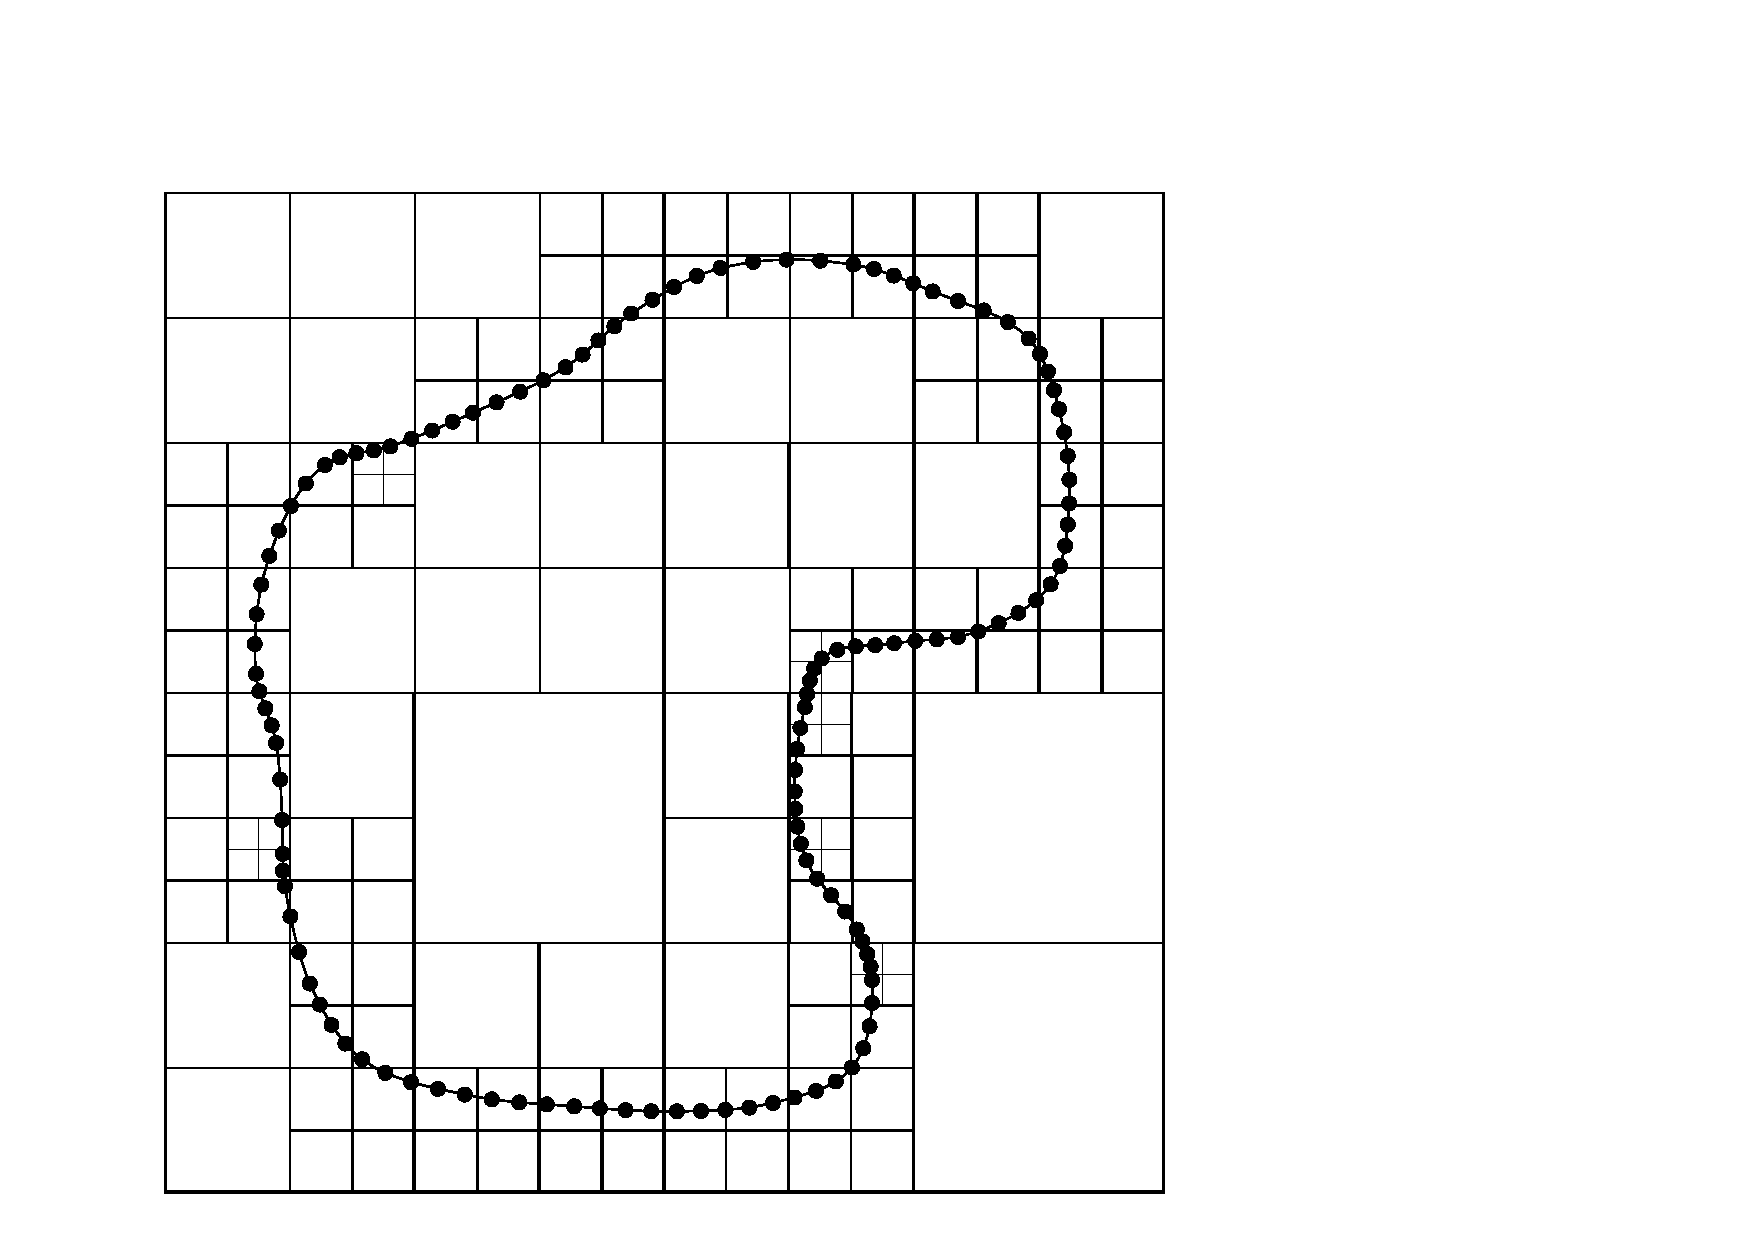
\includegraphics[width=12cm]{img/Quadtree.pdf}
	\caption{Adaptive quadtree in 2 dimensions}
	\label{fig:quadtree}
\end{figure}

The tree structure is then traversed, summing influences of near clusters directly (particle-particle) and evaluating the multipole approximations of distant clusters (cluster-particle). This delineation is controlled by a \emph{multipole acceptance criteria}, where a specified $\theta_{\text{MAC}}$ is compared to $\theta = b/d$, where $d$ is the distance between clusters and $b$ is a function of the size of the interacting clusters. If $\theta < \theta_{\text{MAC}}$ then the interaction is classed as short-range. This approach, represented by figure \ref{fig:treecode} gives a computational complexity of $\bigO(N\log N)$, enabling large calculations to be run in a reasonable timeframe.

\begin{figure}[h]
	\centering
	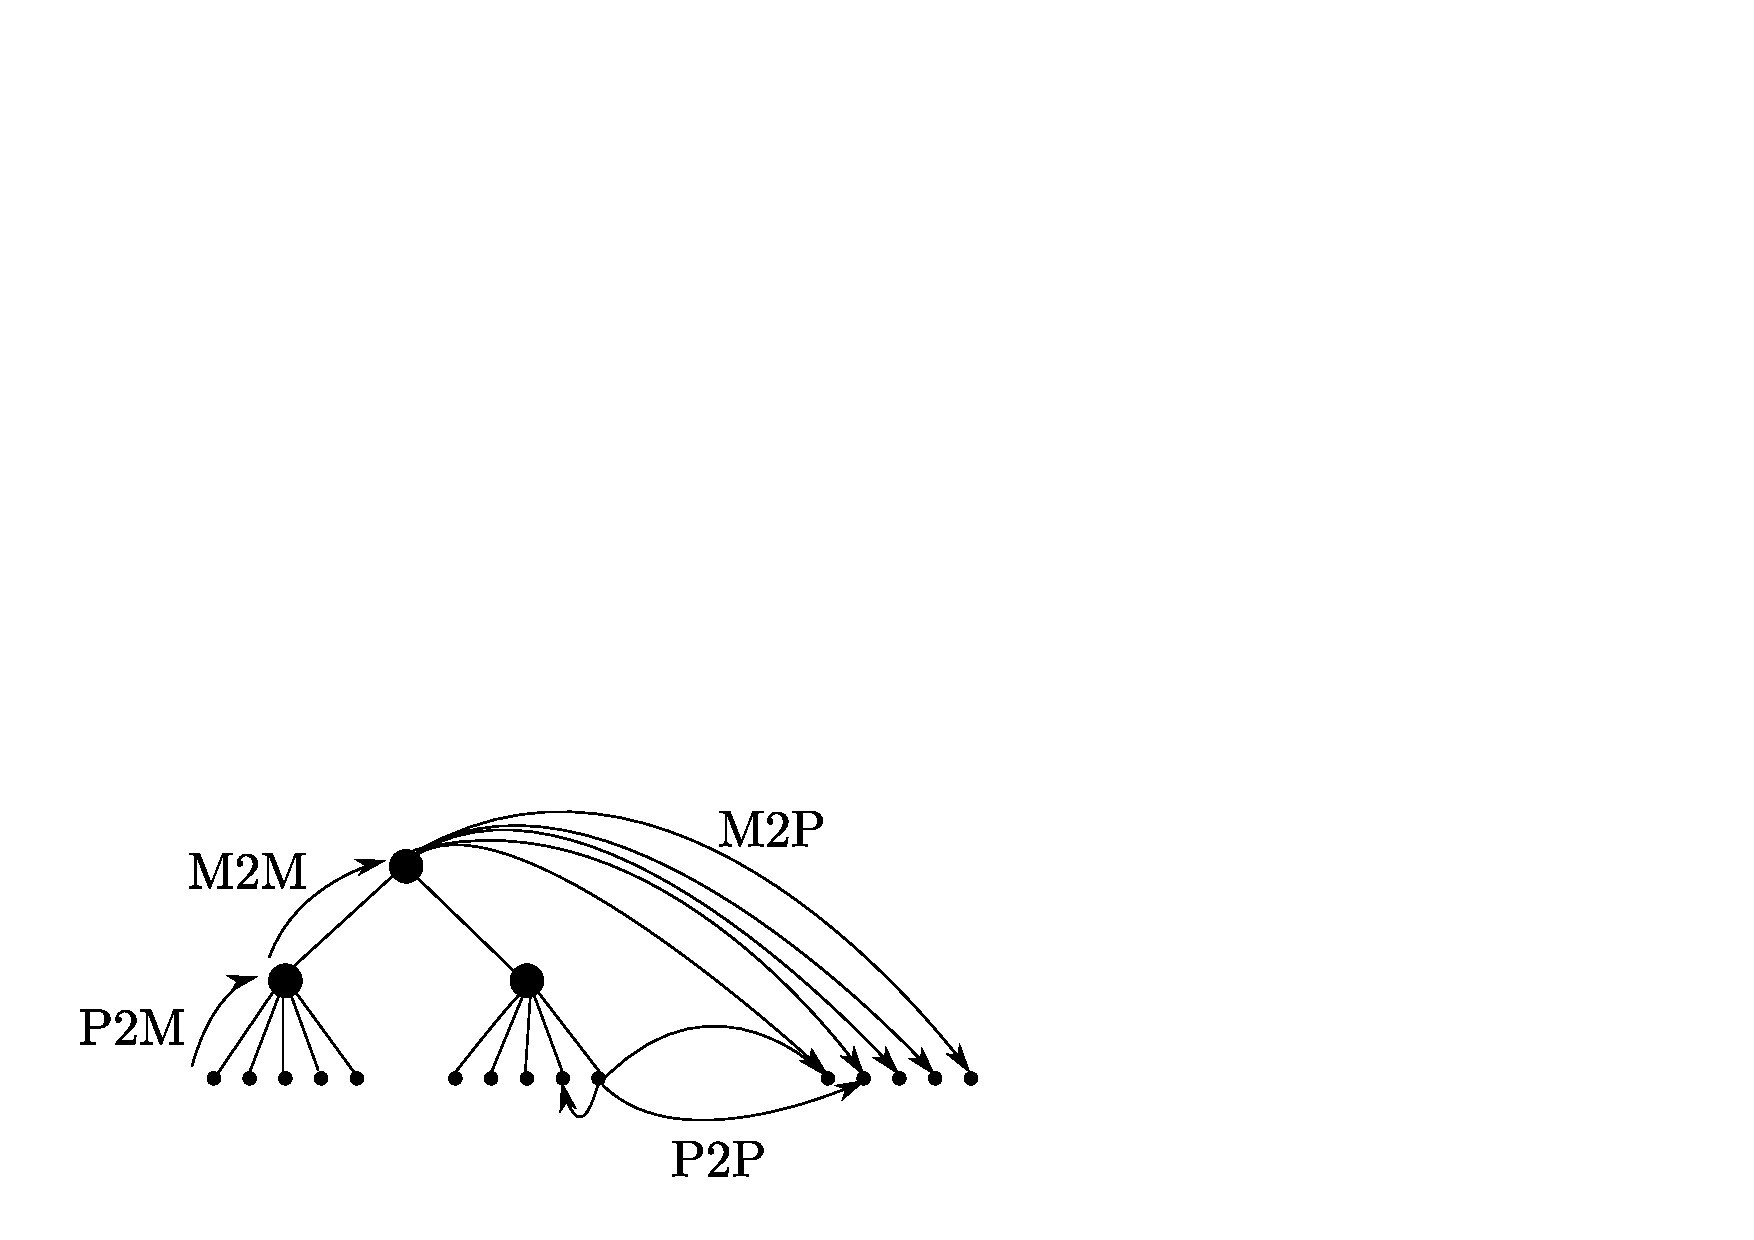
\includegraphics[width=10cm]{img/Treecode.pdf}
	\caption{Treecode}
	\label{fig:treecode}
\end{figure}

This method was later extended into the fast multipole method ({\fmm}) by Greengard \cite{greengard1987} to add local expansions which converge within a short distance of the expansion center. Instead of directly evaluating the multipole expansions of far clusters, the multipoles are translated and converted into local expansions (cluster-cluster), before being translated to the lowest nodes of the tree and evaluated against target points. Due to this modification, the overall complexity was reduced to the optimal $\bigO(N)$. A graphical representation of the algorithm is given in figure \ref{fig:fmm}. Later, support for other kernels, including Yukawa \cite{Boschitsch99,HuangJiaZhang2009} and Helmholtz \cite{GreengardETal1998} were added.

\begin{figure}[h]
	\centering
	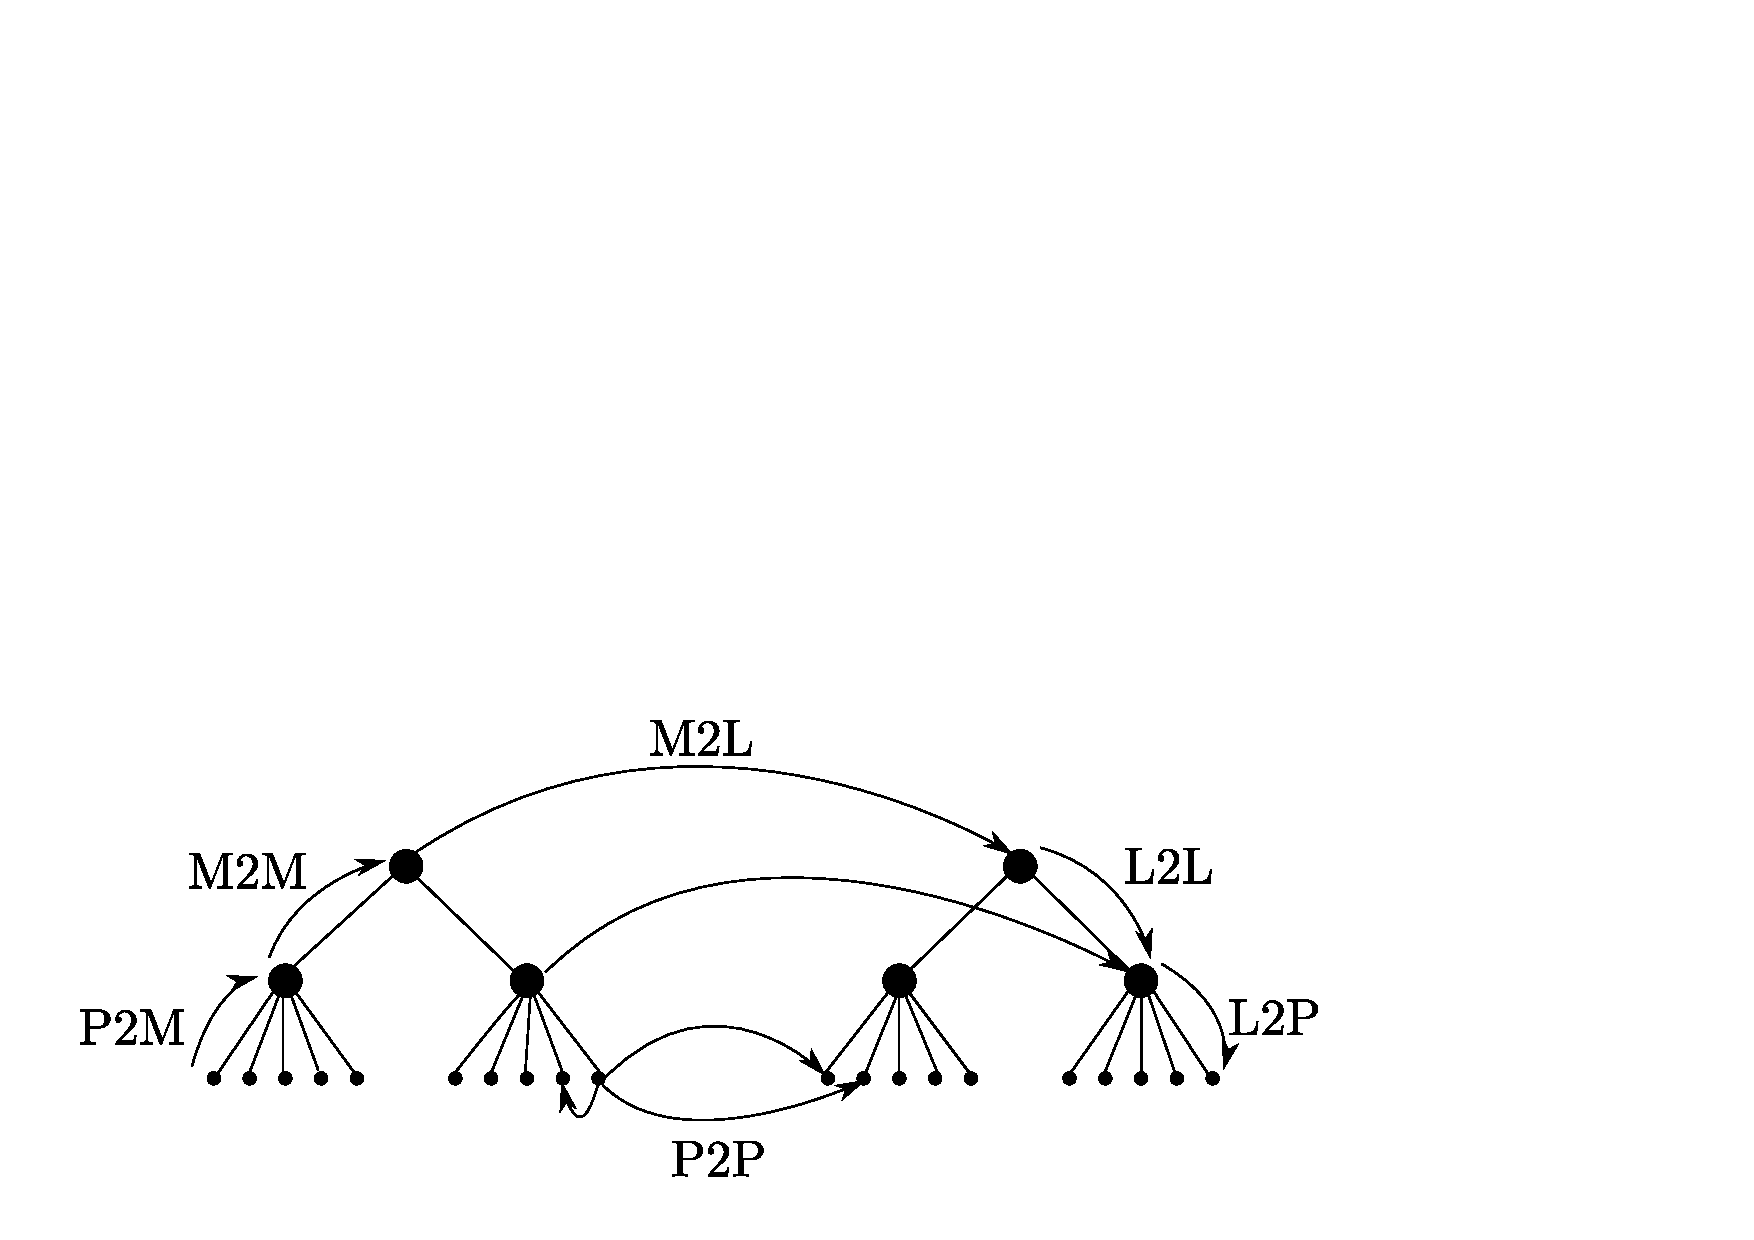
\includegraphics[width=12cm]{img/FMM.pdf}
	\caption{FMM}
	\label{fig:fmm}
\end{figure}

The {\fmm} can be used for any problem that has an n-body sum of the form of equation (\ref{eqn:nbody}) and a suitable Green's function. During each iterative solve step within the {\bem} we repeatedly compute sums of this kind due to evaluating integrals using Gauss quadrature --- repeated Green's function evaluations. Therefore, the {\fmm} can be used to accelerate this process.

{\fmm} and treecodes can be thought of as having 7 separate operators (or kernels) described in \S\ref{subsec:fmm_operators}, and 3 distinct ``phases'', summarised below in \S\ref{subsec:fmm_phases}. How these operators pertain to a tree structure is shown in figures \ref{fig:treecode} and \ref{fig:fmm} for treecodes and {\fmm}s respectively.

%%%%%%%%%%%%
% KERNELS
%%%%%%%%%%%%
\subsection{Operators}\label{subsec:fmm_operators}

There are 7 separate operators that constitute a standard {\fmm}, each performing a distinct operation, from directly evaluating the influence from one particle on another, to creating a multipole expansion, to translating series expansions up, down or across the tree. These operators are summarised below.

\begin{itemize}

\item \emph{Particle to Particle (P2P)} -- Calculate directly (using an $\bigO(N^{2}$) method) the interactions between source and target particles.

\item \emph{Particle to Multipole (P2M)} -- Generate a multipole expansion about a cluster center of all source particles contained within that cluster.

\item \emph{Multipole to Multipole (M2M)} -- Translate a multipole expansion by shifting it to a different center.

\item \emph{Multipole to Particle (M2P)} -- Evaluate a multipole expansion at a \emph{well-separated} target particle.

\item \emph{Multipole to Local (M2L)} -- Translate a multipole expansion to a \emph{well-separated} center point, and convert into a local expansion.

\item \emph{Local to Local (L2L)} -- Translate a local expansion to a different center.

\item \emph{Local to Particle (L2P)} -- Evaluate a local expansion at nearby particles.

\end{itemize}

\subsection{Phases of the FMM}\label{subsec:fmm_phases}

To perform a standard {\fmm}, we require 4 distinct phases, performed in order. Each of these phases is shown below, along with pseudocode for each phase.

\begin{itemize}

\item \emph{Tree Creation}, (algorithm \ref{alg:tree_construction}) -- The domain is partitioned hierarchically based on $N_{\text{CRIT}}$. Links between cells and their parents / children are created at this point for fast traversal later.

\begin{algorithm}
	\caption{Tree Construction}
	\label{alg:tree_construction}
	\begin{algorithmic}
		\Require Maximum \# of particles per cluster NCRIT, root cluster
		\State root = root\_cluster
		\For{sources, $j$}
			\State \Call{add\_to\_cluster}{$j$, root}
		\EndFor
		\State
		\Procedure{add\_to\_cluster}{point, cluster}
			\If{\Call{num\_points}{cluster} $<$ NCRIT}
				\State cluster.\Call{append}{point}
			\Else
				\If{not cluster.split}
					\State \Call{split}{cluster} \Comment Split into 8 child clusters
				\EndIf
				\State oct = \Call{octant}{point, cluster} \Comment Get correct child cluster
				\State \Call{add\_to\_cluster}{point, cluster.child[oct]}
			\EndIf
		\EndProcedure
	\end{algorithmic}
\end{algorithm}

\item \emph{Upward}, (algorithm \ref{alg:upward_sweep}) -- Multipole expansions are created at all leaf (lowest level) clusters (P2M). Then, expansions are translated up the tree to parent clusters (M2M). At the end of this stage, all clusters contain a multipole representation of all particles approximated by themselves and their descendants.

\begin{algorithm}
	\caption{Upward sweep}
	\label{alg:upward_sweep}
	\begin{algorithmic}
		\Require Cells $C$, kernel $K$.
		\For{i=1,\;...,\;\Call{size}{$C$}}
			\If{\Call{is\_leaf}{$C_{i}$}} 
				\State \Call{K.P2M}{points($C_{i}$)} \Comment Create multipole expansions at leaf cells
			\Else
				\State \Call{K.M2M}{$C_{i}$,\;parent($C_{i}$)}\Comment Translate multipole expansions up the tree
			\EndIf
		\EndFor
	\end{algorithmic}
\end{algorithm}

\item \emph{Interaction}, (algorithm \ref{alg:interaction}) -- Both long and short range interactions are calculated, based on interacting source and target clusters against each other. If the ratio $\theta = b / d$, where $d$ is the distance between 2 cluster centers, and $b$ is a function of the cluster sizes is less than some specified $\theta_{\text{MAC}}$, then direct particle-particle (P2P) evaluation is used. Otherwise, either cluster-particle (M2P) in the case of a treecode, or cluster-cluster (M2L) operators in the case of an {\fmm} are evaluated.

\begin{algorithm}
	\caption{Interaction Stage}
	\label{alg:interaction}
	\begin{algorithmic}
		\State pairQ = [\Call{root}{source}, \Call{root}{target}]
		
		\While{not \Call{empty}{pairQ}}
			\State pair = \Call{pop\_front}{pairQ}
			\State $b_{1}, b_{2}$ = pair.first, pair.second
			\If{\Call{is\_leaf}{$b_{1}$}}
				\If{\Call{is\_leaf}{$b_{2}$}} \Comment Both leaves -- direct evaluation
					\State \Call{P2P}{$b_{1}, b_{2}$}
				\Else
					\For{$bc$ in \Call{children}{$b_{2}$}}
						\State \Call{interact}{$b_{1}, bc$}
					\EndFor
				\EndIf
			\ElsIf{\Call{is\_leaf}{$b_{2}$}}
				\For{$bc$ in \Call{children}{$b_{1}$}}
					\State \Call{interact}{$bc,b_{2}$}
				\EndFor
			\Else
				\State \Call{interact}{...} \Comment Iterate over smaller box's children
			\EndIf
		\EndWhile
		\State
		\Procedure{interact}{$\text{Box}_{1}, \text{Box}_{2},$ pairQ} \Comment Interact two boxes
			\If{\Call{accept\_mac}{$\text{Box}_{1}, \text{Box}_{2}$}} \Comment Long-range interactions
				\If{FMM} 
					\State \Call{M2L}{$\text{Box}_{1}, \text{Box}_{2}$} \Comment Translate and convert multipole expansion
				\EndIf
				\If{TREECODE} 
					\State \Call{M2P}{$\text{Box}_{1}, \text{Box}_{2}$} \Comment Evaluate multipole at far points
				\EndIf
			\Else{}
				\State pairQ.\Call{push\_back}{pair($\text{Box}_{1}, \text{Box}_{2}$)} \Comment Not accepted, defer for splitting
			\EndIf
		\EndProcedure
	\end{algorithmic}
\end{algorithm}

\item \emph{Downward}, (algorithm \ref{alg:downward_sweep}) -- For a treecode, this phase is empty. For an {\fmm}, local expansions are propagated downwards through the tree (L2L), passing from a parent cluster to its children. At the leaf nodes, these local expansions are evaluated at all target points within each relevant cluster (L2P).

\begin{algorithm}
	\caption{Downward Sweep}
	\label{alg:downward_sweep}
	\begin{algorithmic}
		\For{all clusters, $c$}
			\If{not \Call{is\_leaf}{$c$}}
				\For{$ci$ in \Call{children}{$c$}}
					\State \Call{L2L}{$c, ci$} \Comment Translate local expansions down the tree
				\EndFor
			\Else{}
				\State \Call{L2P}{$c$} \Comment Evaluate local expansions at leaf cells
			\EndIf
		\EndFor
	\end{algorithmic}
\end{algorithm}
	
\end{itemize}

%%%%%%%%%%%%
% COMPLEXITY
%%%%%%%%%%%%
\subsection{Computational Complexity}

While we've already stated that the {\fmm} has $\O{N}$ scaling, we will now demonstrate it by breaking down the algorithm into distinct sections, giving the complexity of each section and thus the total complexity.

First of all, we define some useful values:

\begin{center}
\begin{tabular}{c|c}
	$N$ & Number of particles \\
	$l$ & Number of levels in the Octree, $\approx \log_8N$ \\
	$p$ & Truncation point of expansions \\
	$c_{\text{P2M}}(p)$ & Cost of a creating multipole expansion (single source) \\
	$c_{\text{M2M}}(p)$ & Cost of a single multipole-multipole translation \\
	$c_{\text{M2L}}(p)$ & Cost of a single multipole-local translation \\
	$c_{\text{L2L}}(p)$ & Cost of a single local-local translation \\
	$c_{\text{L2P}}(p)$ & Cost of evaluating a local expansion (single target) \\
	$N_{\text{M2L}}$ & Number of {\mtol} translations ($=189$)
	%$n$ & Cost of direct particle-particle between 2 boxes
\end{tabular}
\end{center}

Using these, we can form an estimate for the total runtime of the {\fmm} in terms of the cost of our expansions, which will then be specialized for a pair of different expansion types.
\begin{eqnarray}
	C_{\text{\fmm}} & = & N\cdot c_{\text{P2M}}(p) \nonumber \\
	& + & N\cdot c_{\text{M2M}}(p) \nonumber \\
 	& + & N\cdot N_{\text{M2L}}\cdot c_{\text{M2L}}(p) \label{eqn:fmm_costs} \\
	& + & N\cdot c_{\text{L2L}}(p) \nonumber \\
	& + & N\cdot c_{\text{L2P}}(p) \nonumber \\
	& + & N\cdot 27\cdot N_{\text{CRIT}}^{2} \nonumber
\end{eqnarray}

Clearly this shows that the total complexity is $\O{N}$ as long as $p \not= p(N)$, something that holds for all applications discussed in this thesis, and $\ncrit \ll N$, which holds for any reasonably created tree. (A notable application where $p = p(N)$ would be acoustics, using expansions for the Helmholtz Green's function). With a standard $\fmm$ formulation, $N_{\text{M2L}} = 189$. We can look at two examples, firstly Cartesian expansions, equation (\ref{eqn:cartesian_multipole})

\begin{equation}
	\phi(\vect{x}_i) = \sum_{||\vect{k}||=0}^{\vect{P}}\frac{1}{\vect{k}!}D^{k}_y(\vect{x_i},\vect{y})\psi(\vect{y}_j-\vect{y}_c)^{\vect{k}},
	\label{eqn:cartesian_multipole}
\end{equation}

where $\vect{k}$ is a multi-index variable, $\vect{k}=\{k_1, k_2, k_3\}$, $\vect{k}! = k_1!k_2!k_3!$, $\vect{y}^{k} = y_1^{k_1}y_2^{k_2}y_3^{k_3}$ and $D_y^{k} = D^{k_1}_{y_1}D^{k_2}_{y_2}D^{k_3}_{y_3}$ is the derivative operator. The other expansion we use as an example are spherical harmonic expansions, shown for Laplace's equation in equation (\ref{eqn:spherical_multipole}).

\begin{equation}
\phi(\vect{x}_i) = \sum_{n=0}^{p}\sum_{m=-n}^{n}\frac{Y^{m}_n(\theta_i,\phi_i)}{r_i^{n+1}}\left \{\sum_j^{N}q_j\rho^{n}_jY^{-m}_n(\alpha_i,\beta_i)\right \}
	\label{eqn:spherical_multipole}
\end{equation}

\begin{center}
	\begin{tabular}{c|c|c}
		Operation & Cost (Cartesian) & Cost (Spherical) \\ \hline
		$c_{\text{P2M}}$ & $\O{p^{3}}$ & $\O{p^{2}}$ \\
		$c_{\text{M2M}}$ & $\O{p^{6}}$ & $\O{p^{4}}$ \\
		$c_{\text{M2L}}$ & $\O{p^{6}}$ & $\O{p^{4}}$ \\
		$c_{\text{L2L}}$ & $\O{p^{6}}$ & $\O{p^{4}}$ \\
		$c_{\text{L2P}}$ & $\O{p^{3}}$ & $\O{p^{2}}$
	\end{tabular}
\end{center}

When we apply these costs to equation (\ref{eqn:fmm_costs}) we can immediately see that the most expensive expansion related cost will be the {\mtol} translations due to the large constant multiplier, given by $N\cdot N_{\text{M2L}}\cdot\O{p^{4}}$ for spherical expansions and $N\cdot N_{\text{M2L}}\cdot\O{p^{6}}$ for cartesian. The other most expensive part of the evaluation will be the direct near-field computation, given by $N\cdot 27\cdot \ncrit^{2}$. The fastest {\fmm} will usually involve trying to create a tree that keeps these two costs as equal as possible, known as \emph{well-balanced}. This balance comes from trying to ensure that $\ncrit$ does not become so large that the algorithm starts to scale as $\O{N^{2}}$, while making sure that the tree does not have so many levels that the number of {\mtol} translations becomes too large and dominates the run time. The high cost of {\mtol} translations is going to be one of the main motivators for the relaxation schemes introduced later in \S\ref{subsec:inexact_matvec}.

\section{Preconditioners}

In all the experiments performed in this work, an important metric is the number of iterations taken by our linear solver to converge to a solution. Given the cost of each iteration, this number will also heavily influence the total time-to-solution. The number of iterations will be most directly influenced by the \emph{condition number} of the matrix, $\kappa(A)$, given here for a normal matrix

\begin{equation}
	\kappa(A) = \left | \frac{\lambda_{\text{max}}(A)}{\lambda_{\text{min}}(A)} \right |,
\end{equation}

\noindent
where $\lambda_{\text{max}}$ and $\lambda_{\text{min}}$ are the largest and smallest eigenvalues of $A$ respectively. As the ratio of these eigenvalues gets closer to $1$, the matrix becomes more \emph{well-conditioned} and easier to solve (i.e. less solver iterations are needed).

In the context of Krylov solvers, one way to try and reduce the condition number is to apply a preconditioner, indicated in algorithm \ref{alg:gmres} by the step $Mz_j = v_j$ or

\begin{equation}
	z_{j} \gets M^{-1}\cdot v_{j},
\end{equation}

\noindent
with $M$ as some approximation to $A$. A simple example of $M$ is simply the diagonal of $A$, that is,

\begin{equation}
	M(A) = \text{diag}(A)
\end{equation}

%Note that the preconditioner, $M^{-1}$ can be thought of as a linear operator which operates on a vector. We can write this in a general form as $M^{-1}(x)$. This allows us to substitute any linear operator that will improve the solution as the operator $M^{-1}$. A simple example of this would be a diagonal preconditioner:
%
%\begin{equation}
%	M^{-1}(x) = \frac{x}{\text{diag}(A)}.
%\end{equation}

In this case, we can explicitly form $M^{-1}$, and applying the preconditioner is a simple element-wise multiplication between $M^{-1}$ and $v_j$ (\lstinline|axpy| in standard dense linear algebra notation). 

In general we may have to solve the $Mz_j = v_j$ system using a choice of linear solver (including another Krylov solver). The only additional overhead for this kind of so-call ``flexible'' preconditioner \cite{saad1993} from the viewpoint of the {\gmres} solver,  is a slightly increased memory footprint. There are multiple ways of modifying {\gmres} to accommodate this type of preconditioning; The one used in this thesis is {\fgmres}, algorithm \ref{alg:fgmres} \cite{saad1993}, simply {\gmres} as described in algorithm \ref{alg:gmres}, with two small changes: $V_{k} \gets [v_{1},...,v_{k}]$ changes to $Z_{k} \gets [z_{1},...,z_{k}]$ and we use $Z_{k}$ instead of $V_{k}$ when updating the approximation $x_{k}$. The {\fgmres} algorithm is shown in pseudocode as algorithm \ref{alg:fgmres}.

\begin{algorithm}
	\caption{Right-Preconditioned FGMRES \cite{saad1993}}
	\label{alg:fgmres}
	\begin{algorithmic}
		\Require Matrix $A$, initial guess $x_{0}$, right-hand side $b$, desired tolerance $\epsilon$, order of the Krylov space $k$, preconditioner $M$.
		\State Initialize $\bar{H}_{m} \in \R^{(k+1)\times k} = 0\;\forall i,j$
		\State $r_{0} \gets A\cdot x_{0}-b$
		\State $\beta \gets ||r_{0}||_{2},\;\; v_{1} \gets r_{0}/\beta$
		\For{j=1,...,k}
			\State $z_{j} \gets M^{-1}\cdot v_{j}$
			\State $w \gets A\cdot z_{j}$
			\For{i=1,..,j}
				\State $h_{i,j} \gets (w, v_{i})$
				\State $w \gets w - h_{i,j}\cdot v_{i}$
			\EndFor
			\State $h_{j+1,j} \gets ||w||_{2}$
			\State $v_{j+1} \gets w / h_{j+1,j}$
		\EndFor
		\State $Z_{k} \gets \left [z_{1}, ..., z_{k} \right]$
		\State $y_{k} = \arg\min_{y}||\beta e_{1} - \bar{H}_{k}y||_{2}$ and $e_{1} = [1,0,...,0]$
		\State $x_{k} \gets x_{0} + Z_{k}y_{k}$ 
	\end{algorithmic}
\end{algorithm}

Notice that the main cost per iteration is still the matvec $w \gets A\cdot z_{j}$, so the additional overhead of using the {\fgmres} variant is insignificant.

\section{Inexact Matrix-Vector Products}\label{subsec:inexact_matvec}

Consider the case where a matrix-vector product is not computed exactly, such as when using {\fmm} within {\gmres} or {\fgmres}. In this situation, $y \gets A\cdot x$ becomes $y \gets (A+\epsilon_{A})\cdot x$ with $\epsilon_A$ representing the errors induced by the {\fmm} approximation. It can be shown \cite{simonciniszyld2003} that not only will we still converge to the correct solution of the linear system, but that $||\epsilon_{A}||$ can grow as the residual becomes closer to the final desired tolerance. 

By introducing an error term on the $i$-th iteration to our matrix $A$, $E_i$, instead of the standard Arnoldi iteration used in {\gmres}, $AV_m = V_{m+1}H_{m}$, where $H_m$ is the upper-Hessenberg matrix produced from the Arnoldi iterations and $V_m = [v_1, v_2, \cdots, v_m]$, we use the \emph{inexact Arnoldi} iteration,

\begin{equation}
	[(A+E_1)v_1, \cdots, (A+E_m)v_m] = [v_1, \cdots, v_m]H_m.
\end{equation}

Assuming that the calculation of the initial residual, $r_0 = b-Ax_0$ is exact, and $\beta = ||r_0||$, we can write the $m$-th iteration of the {\gmres} procedure as $x_m = x_0 + \delta_mx$, with $\delta_mx = V_my_m$ and $y_m$ is the solution to $\min_y||H_my-\beta e_1||$. We diverge from the standard exact {\gmres} by introducing a perturbation matrix, $G_m = [E_1v_1, \cdots, E_mv_m]$. From here, we can write the inexact Arnoldi iteration as an exact Arnoldi iteration with

\begin{equation}
	(A+G_m V_m^{T})V_m = V_{m+1}H_m
\end{equation}

This shows that the quantities calculated in the first $i$ steps of an inexact Arnoldi iteration are exactly the same as the first $i$ steps of an exact iteration with $A = (A+G_mVM^{T})$. From this, we can use the standard {\gmres} results to show that the residual $r_m$ will decrease as $i$ grows, establishing the convergence of our inexact {\gmres}.

The convergence of an inexact {\gmres} solver has also been shown experimentally for dense linear algebra \cite{vandeneshofsleijpen2004,bourasfraysse2005,simonciniszyld2003}, and was implemented by explicitly adding a perturbation to $A$, such that $A' \gets A + A_\epsilon$ and $||A_\epsilon||$ is controlled as part of the relaxation strategy. A different approach \cite{sidjewinkles2011} has been used for sparse matrices, namely specifiying a ``drop-tolerance'', $\epsilon$, where if $||A_{ij}|| \leq \epsilon$, then that term is not counted when performing the matrix-vector products within {\gmres}.

We take a different approach with the {\fmm}, given that we can control error by using $p$ and $\theta_{\text{MAC}}$ as described in \S\ref{sec:fmm}. Given these values it is natural that we use them to adjust the accuracy of the {\fmm} for each iteration, reducing the accuracy to perform the minimum amount of work necessary, speeding up the calculation. We expect this to give a speedup due to the scaling of the {\fmm} --- the two main contributions to the {\fmm}'s runtime are, from \S\ref{sec:fmm}, the near-field calculation between boxes, taking $N\cdot27\cdot\ncrit^{2}$ time, and the {\mtol} translation stage, which takes $N\cdot N_{\text{M2L}}\cdot c_{\text{M2L}}(p)$ time. Given that $c_{\text{M2L}}(p) = \O{p^{4}}$ for a standard spherical harmonics expansion and $\O{p^{6}}$ for Cartesian series, the reduction in time can be significant as $p$ is reduced. For example, moving from $p = 10$ to $p=1$ is a potential $10^{4}\times$ reduction in work for the spherical harmonics case. While this level of acceleration is unlikely to be obtained in practise it shows the potential of reducing $p$ throughout the process of an iterative solve.

% The {\fmm} can control its error using the properties $p$ and $\theta_{\text{MAC}}$ described in \S\ref{sec:fmm}, so it is natural to take advantage, adjusting the accuracy of the {\fmm} for each iteration, in order to perform the minimum amount of work necessary, thus speeding up the calculation.

This method of controlling (and increasing) induced errors throughout the iterations of a linear solve is known as a \emph{relaxation scheme}. In chapter \ref{chapter:methods} we will describe the exact nature of a relaxation scheme, and look at the remaining numerical methods that will be used in order to perform experiments on a variety of sample {\bem} problems to demonstrate the application of relaxation schemes for {\fmmbem}. These experiments will constitute the first such work with relaxation schemes and {\fmmbem} solvers.

%We will now use these methods to perform experiments on a sample {\bem} problem, evaluating both the convergence of {\fmm}-{\bem}, and the effectiveness of our implemented preconditioners and relaxation strategies.
